\documentclass[tikz,border=2pt]{standalone}
\usepackage[T1]{fontenc}
\usepackage{helvet,amsmath,amssymb,fix-cm}
\renewcommand{\familydefault}{\sfdefault}
\usetikzlibrary{arrows.meta,calc,positioning,fit,backgrounds,decorations.pathreplacing,shapes.geometric}
\definecolor{ink}{HTML}{243343}
\definecolor{physical}{HTML}{3478A3}
\definecolor{semantic}{HTML}{B27C26}
\definecolor{feasible}{HTML}{248679}
\definecolor{decode}{HTML}{75609D}
\definecolor{fault}{HTML}{BA5554}
\definecolor{muted}{HTML}{6F7D88}
\tikzset{
  every node/.style={font=\fontsize{9}{10.8}\selectfont,text=ink},
  edge/.style={-{Stealth[length=1.8mm,width=1.25mm]},line width=.6pt,draw=ink},
  param/.style={-{Stealth[length=1.7mm]},line width=.6pt,draw=decode,dashed},
  link/.style={line width=.8pt,draw=physical},
  reject/.style={line width=.7pt,draw=fault,dashed},
  panel/.style={rounded corners=2pt,draw=muted!45,line width=.45pt,fill=white},
  box/.style={rounded corners=2pt,draw=physical!70,line width=.55pt,fill=physical!6,align=center,inner sep=3pt},
  sem/.style={box,draw=semantic!70,fill=semantic!8},
  gate/.style={box,draw=feasible!70,fill=feasible!7},
  dec/.style={box,draw=decode!70,fill=decode!7},
  tinylabel/.style={font=\fontsize{8}{9.4}\selectfont},
  smalllabel/.style={font=\fontsize{8.5}{10}\selectfont},
  heading/.style={font=\bfseries\fontsize{10}{11.5}\selectfont,anchor=north west},
  dot/.style={circle,minimum size=.43cm,inner sep=0pt,draw=physical,fill=white,line width=.8pt,font=\bfseries\fontsize{9}{10}\selectfont},
  receiver/.pic={\draw[draw=physical,line width=.8pt] (0,0)--(0,.58) (-.17,0)--(.17,0) (-.15,.39)--(0,.58)--(.15,.39);
    \draw[draw=physical!70,line width=.55pt] (-.2,.56) arc[start angle=160,end angle=200,radius=.23];
    \draw[draw=physical!70,line width=.55pt] (.2,.40) arc[start angle=-20,end angle=20,radius=.23];},
}
\begin{document}
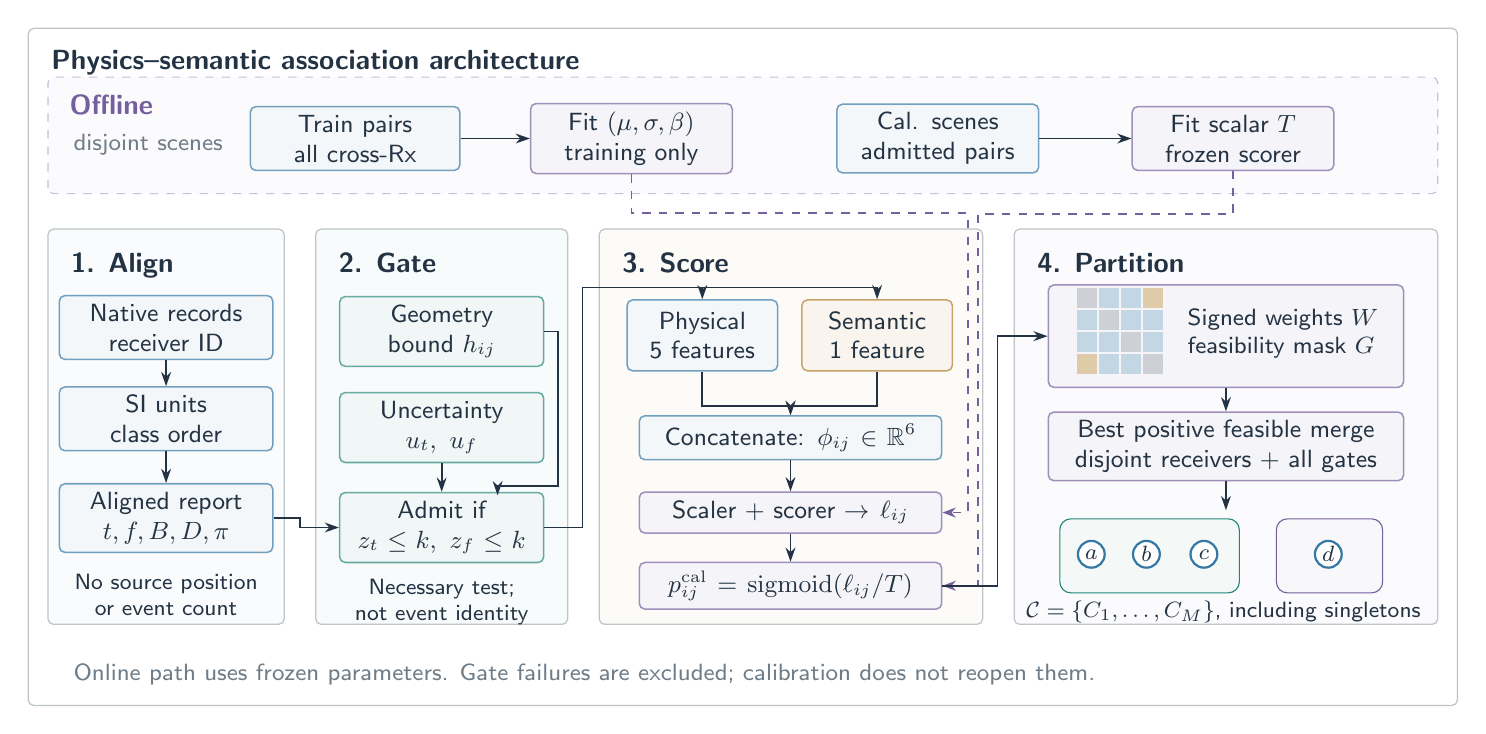
\begin{tikzpicture}[x=1cm,y=1cm]
\draw[panel] (0,0) rectangle ++(18.15,8.6);
\node[heading] at (0.17,8.45) {Physics--semantic association architecture};

\draw[rounded corners=2pt,draw=decode!40,fill=decode!3,dashed] (.25,6.5) rectangle (17.9,7.98);
\node[heading,text=decode] at (.4,7.87) {Offline};
\node[box,text width=2.45cm,minimum height=.75cm] (train) at (4.15,7.2) {Train pairs\\all cross-Rx};
\node[dec,text width=2.35cm,minimum height=.75cm] (fit) at (7.66,7.2) {Fit $(\mu,\sigma,\beta)$\\training only};
\node[box,text width=2.35cm,minimum height=.75cm] (cal) at (11.55,7.2) {Cal. scenes\\admitted pairs};
\node[dec,text width=2.35cm,minimum height=.75cm] (temp) at (15.3,7.2) {Fit scalar $T$\\frozen scorer};
\draw[edge] (train)--(fit); \draw[edge] (cal)--(temp);
\node[smalllabel,anchor=west,text=muted] at (.45,7.12) {disjoint scenes};

\draw[panel,fill=physical!3] (.25,1.03) rectangle (3.25,6.05);
\draw[panel,fill=feasible!3] (3.65,1.03) rectangle (6.85,6.05);
\draw[panel,fill=semantic!3] (7.25,1.03) rectangle (12.12,6.05);
\draw[panel,fill=decode!3] (12.52,1.03) rectangle (17.9,6.05);
\node[heading] at (.42,5.87) {1. Align};
\node[heading] at (3.82,5.87) {2. Gate};
\node[heading] at (7.42,5.87) {3. Score};
\node[heading] at (12.69,5.87) {4. Partition};

\node[box,text width=2.5cm,minimum height=.65cm] (records) at (1.75,4.80) {Native records\\receiver ID};
\node[box,text width=2.5cm,minimum height=.73cm] (canonical) at (1.75,3.64) {SI units\\class order};
\node[box,text width=2.5cm,minimum height=.74cm] (obs) at (1.75,2.38) {Aligned report\\$t,f,B,D,\pi$};
\draw[edge] (records)--(canonical); \draw[edge] (canonical)--(obs);
\node[tinylabel,align=center,text width=2.5cm] at (1.75,1.4) {No source position\\or event count};

\node[gate,text width=2.38cm,minimum height=.75cm] (bound) at (5.25,4.75) {Geometry\\bound $h_{ij}$};
\node[gate,text width=2.38cm,minimum height=.75cm] (unc) at (5.25,3.53) {Uncertainty\\$u_t,\ u_f$};
\node[gate,text width=2.38cm,minimum height=.75cm] (gate) at (5.25,2.26) {Admit if\\$z_t\leq k,\ z_f\leq k$};
\draw[edge] (bound.east)--(6.73,4.75)--(6.73,2.79)--(5.96,2.79)--(5.96,2.67);
\draw[edge] (unc)--(gate);
\draw[edge] (obs.east)--(3.45,2.38)|-(gate.west);
\node[tinylabel,align=center,text width=2.7cm] at (5.25,1.32) {Necessary test;\\not event identity};

\node[box,text width=1.70cm,minimum height=.9cm] (phys) at (8.56,4.70) {Physical\\5 features};
\node[sem,text width=1.70cm,minimum height=.9cm] (sem) at (10.78,4.70) {Semantic\\1 feature};
\node[box,text width=3.63cm,minimum height=.52cm] (six) at (9.68,3.40) {Concatenate: $\phi_{ij}\in\mathbb R^6$};
\node[dec,text width=3.63cm,minimum height=.52cm] (score) at (9.68,2.45) {Scaler + scorer $\rightarrow\ell_{ij}$};
\node[dec,text width=3.63cm,minimum height=.52cm] (prob) at (9.68,1.52) {$p^{\mathrm{cal}}_{ij}=\mathrm{sigmoid}(\ell_{ij}/T)$};
\draw[edge] (phys.south)--(8.56,3.8)-|(six.north);
\draw[edge] (sem.south)--(10.78,3.8)-|(six.north);
\draw[edge] (six)--(score); \draw[edge] (score)--(prob);
\draw[edge] (gate.east)--(7.04,2.26)--(7.04,5.31)-|(phys.north);
\draw[edge] (7.04,5.31)-|(sem.north);
\draw[param] (fit.south)--(7.66,6.25)--(11.93,6.25)--(11.93,2.45)--(score.east);
\draw[param] (temp.south)--(15.3,6.24)--(12.06,6.24)--(12.06,1.52)--(prob.east);

\node[dec,text width=4.3cm,minimum height=1.3cm] (signed) at (15.21,4.69) {};
\foreach \rr in {0,...,3} \foreach \cc in {0,...,3} {
 \pgfmathsetmacro{\xx}{13.32+.28*\cc}\pgfmathsetmacro{\yy}{4.21+.28*\rr}
 \fill[physical!30] (\xx,\yy) rectangle ++(.25,.25);
}
\foreach \dd in {0,...,3}{\pgfmathsetmacro{\xx}{13.32+.28*\dd}\pgfmathsetmacro{\yy}{4.21+.28*(3-\dd)}\fill[muted!35] (\xx,\yy) rectangle ++(.25,.25);}
\fill[semantic!40] (14.16,5.05) rectangle ++(.25,.25);
\fill[semantic!40] (13.32,4.21) rectangle ++(.25,.25);
\node[anchor=west,align=left,text width=2.55cm,smalllabel] at (14.6,4.72) {Signed weights $W$\\feasibility mask $G$};
\node[dec,text width=4.3cm,minimum height=.85cm] (merge) at (15.21,3.29) {Best positive feasible merge\\disjoint receivers + all gates};
\draw[edge] (prob.east)--(12.31,1.52)--(12.31,4.69)--(signed.west);
\draw[edge] (signed)--(merge);
\draw[edge] (merge.south)--(15.21,2.48);
\draw[rounded corners=4pt,draw=feasible,fill=feasible!5] (13.1,1.43) rectangle (15.38,2.37);
\foreach \xx/\lab in {13.5/a,14.2/b,14.93/c} \node[dot,minimum size=.34cm,tinylabel] at (\xx,1.92) {$\lab$};
\draw[rounded corners=4pt,draw=decode,fill=decode!5] (15.85,1.43) rectangle (17.2,2.37);
\node[dot,minimum size=.34cm,tinylabel] at (16.51,1.92) {$d$};
\node[tinylabel] at (15.18,1.19) {$\mathcal C=\{C_1,\ldots,C_M\}$, including singletons};
\node[smalllabel,anchor=west,text=muted] at (.45,.39)
 {Online path uses frozen parameters. Gate failures are excluded; calibration does not reopen them.};
\end{tikzpicture}
\end{document}
